\section{Create Java interface of CBLAS with JNI}
\label{sec:history}
\begin{enumerate}
    \item Download BLAS and build using make file. In the figure2.1, the built file is libblas.a and the header file is blas.h.
    \item Download CBLAS and build using make file (I am not sure whether we should build archive file or shared library). In figure, the build file would be libcblas.a or libcblas.dylib and header file is cblas.h.
    \item Create java file which will be the Java interface of CBLAS.
    \item Compile java file with -h header flag to create class file (CBLASJ.class) and header file (CBLASJ.h).
\begin{lstlisting}[language=bash]
    $ javac -h . CBLASJ.java
\end{lstlisting}
    \item Create C file (CBLASJ.c) which will bind Java interface and CBLAS library. And compile it with JNI to create object file (CBLASJ.o).
\begin{lstlisting}[language=bash]
    $ gcc -c-fPIC -I${JAVA_HOME}/include -I${JAVA_HOME}/include/darwin CBLASJ.c
\end{lstlisting}
    \item Compile shared library linking library (libcblas.a or libcblas.dylib) object file (CBLASJ.o).
\begin{lstlisting}[language=bash]
    $ gcc -o libcblas.dylib (or libcblas.a) CBLASJ.o 
\end{lstlisting}
\end{enumerate}

\begin{figure}[htb]
    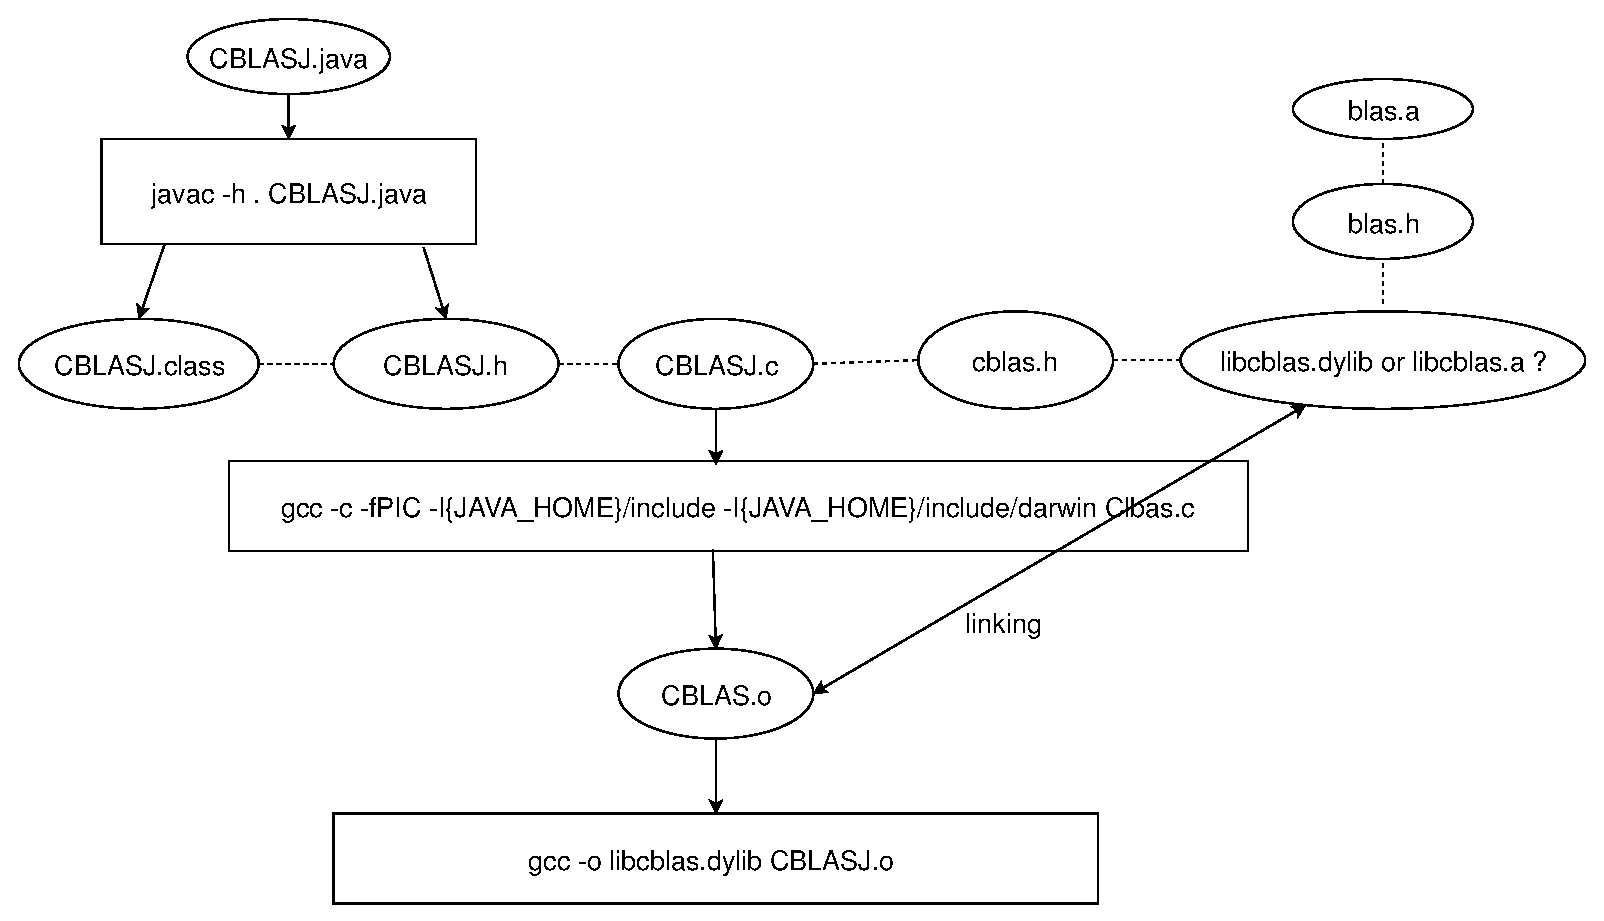
\includegraphics[width=15cm]{cblas_with_jni.eps}
    \caption{Integration of Native Methods }
    \label{fig:Sampling}
\end{figure}

